\PassOptionsToPackage{table}{xcolor}
\documentclass[FP,DP]{tulthesis}
%\hypersetup{
  %  hidelinks = true,
%}
%\usepackage{hyperref}
\usepackage{blindtext}
\usepackage{booktabs}
\usepackage{url}
\usepackage[obeyFinal]{easy-todo}
\usepackage{polyglossia}
\usepackage{enumitem}
\usepackage{array}
\newcolumntype{L}[1]{>{\raggedright\let\newline\\\arraybackslash\hspace{0pt}}m{#1}}
\newcolumntype{C}[1]{>{\centering\let\newline\\\arraybackslash\hspace{0pt}}m{#1}}
\newcolumntype{R}[1]{>{\raggedleft\let\newline\\\arraybackslash\hspace{0pt}}m{#1}}
\usepackage{tikz}
\usepackage{graphicx}
\usepackage{svg}
\usepackage{fancyvrb}
\usepackage{tabularx}
\usepackage{multirow}
\usepackage{array,booktabs}
\usepackage{threeparttable}
\usepackage{csquotes}

\def\UrlBreaks{\do\/\do-}

\setdefaultlanguage{czech}

% bibliografie
\usepackage{natbib}
\bibliographystyle{agsm}
%\setcitestyle{round,aysep={},yysep={;},aysep={,}}



% fonty
\usepackage{fontspec}
\usepackage{xunicode}
\usepackage{xltxtra}
%\setmainfont[Mapping=tex-text,BoldFont={* Bold},Numbers=OldStyle]{Baskerville 10 Pro}
%\setsansfont[Mapping=tex-text,BoldFont={* Bold},Numbers=OldStyle]{Myriad Pro}
%\setmonofont[Scale=MatchLowercase]{Vida Mono 32 Pro} ah

%TIKZ
\usetikzlibrary{calc,trees,positioning,arrows,chains,shapes.geometric,%
    decorations.pathreplacing,decorations.pathmorphing,shapes,%
    matrix,shapes.symbols}
\tikzstyle{startstop} = [rectangle, rounded corners, minimum width=1cm, minimum height=1cm,text centered, draw=black,text width=2cm,fill=orange!20]
\tikzstyle{io} = [rectangle, rounded corners, minimum width=1cm, minimum height=1cm,text centered, draw=black,text width=2cm,fill=orange!20]
\tikzstyle{process} = [rectangle, minimum width=1cm, minimum height=0.8cm, text centered, draw=black, fill=orange!30,text width=2.5cm]
\tikzstyle{decision} = [rectangle, rounded corners, minimum width=1cm, minimum height=0.8cm,text centered, draw=black,text width=2cm]
\tikzstyle{postup} = [rectangle, rounded corners, minimum width=1cm, minimum height=0.8cm,text centered, draw=black,text width=10cm]
\tikzstyle{arrow} = [thick,->,>=stealth]
\tikzstyle{arrow2} = [thick,-,>=stealth]

% příkazy specifické pro tento dokument
\newcommand{\argument}[1]{{\ttfamily\color{\tulcolor}#1}}
\newcommand{\prikaz}[1]{\argument{\textbackslash #1}}
\newenvironment{myquote}{\begin{list}{}{\setlength\leftmargin\parindent}\item[]}{\end{list}}
\newenvironment{listing}{\begin{myquote}\color{\tulcolor}}{\end{myquote}}
\sloppy

% deklarace pro titulní stránku
\TULtitle{Programování v~pregraduální přípravě učitelů informatiky[verze 16. 5.] }{Programming in undergraduate training of CS teachers}
\TULprogramme{N1101}{Matematika}{Mathematics}
\TULbranch{7504T077}{Učitelství informatiky pro střední školy2}{Teacher training for lower and upper-secondary school, Informatics}
\TULbranch{7504T089}{Učitelství matematiky pro střední školy}{Teacher Training for Upper Secondary Schools, Mathematics}
\TULauthor{Bc. Ondřej Vraštil}
\TULsupervisor{Mgr. Jan Berki, Ph.D.}
\TULyear{2016}


% příkazy
\newcommand{\verze}{1.3}
\newcommand{\chapquote}[3]{\begin{quotation} \textit{#1} \end{quotation} \begin{flushright} - #2, \textit{#3}\end{flushright} }

\newcommand{\ahoj}[2]{\begin{quotation} \textit{#1} \end{quotation} \begin{flushright} - \textit{#2}\end{flushright} }



\usepackage{booktabs}

\begin{document}

\ThesisStart{male}

\begin{abstractCZ}
Tato zpráva popisuje třídu \texttt{tulthesis} pro sazbu absolventských prací
Technické univerzity v~Liberci pomocí typografického systému \LaTeX.
\end{abstractCZ}

\vspace{2cm}

\begin{abstractEN}
This report describes the \texttt{tulthesis} package for Technical university of
Liberec thesis typesetting using the \LaTeX\ typographic system.
\end{abstractEN}

\clearpage

\begin{acknowledgement}
Rád bych poděkoval všem, kteří přispěli ke vzniku tohoto dílka.
\end{acknowledgement}

\tableofcontents

\clearpage

%\begin{abbrList}
%\textbf{TUL} & Technická univerzita v~Liberci \\
%\end{abbrList}
\chapter{Úvod}
Nedílnou součástí pregraduální přípravy budoucích učitelů informatiky základních i~středních škol je výuka programováni a teorie algoritmů. Toto téma je v~současnosti získává na popularitě i na středních a základních školách, kde je mu věnováno stále více pozornosti. Výuka úvodu do programování a algoritmického myšlení je nejen obsažena v~rámcovém vzdělávacím programu pro gymnázia a některé odborné střední školy, ale v~uzpůsobené podobě se objevuje~i ve výuce na školách základních, kde se mohou mladí žáci setkat se speciálními programovacími jazyky pro děti.

Aby mohla být správně provedena didaktická transformace směrem od učiva k~žákovi, musí její původce -- učitel mít dostatečný vhled do problematiky a~ patřičné vzdělání v~příslušném tématu. Jednou z~hlavních premis je kvalitní vzdělání v~rámci pregraduální přípravy, ve které by měl student -- budoucí učitel získat vhled do tématu natolik, aby dokázal obstojně předat znalosti svým žákům.  Protože je informatika mladý a dynamicky se rozvíjející obor, na kvalitu pregraduální přípravy má vliv i~relevance a~aktualita vyučovaných témat. V~dnešní době se na našich základních a~středních školách začínají využívat pro školní prostředí nová témata jako je robotika nebo unplugged teaching, pro která je znalost algoritmizace nutná. Fakulty připravující učitele informatiky by měly pružně reagovat na moderní trendy ve výuce a uspokojit poptávku studentů po kvalitním a hlavně využitelném vzdělání, které budou moci využít ve své budoucí praxi,nehledě na to, že z~některých studentů se mohou stát i vysokoškolští pedagogové.  

Jak si naše vysoké školy vedou ve výuce programování a algoritmizace? Následují moderní trendy a požadavky zaměstnavatelů budoucích absolventů? Je pořadí předmětů během studia smysluplné? Dá se vysledovat podobnost mezi programy napříč republikou? Existuje  jeden nejvhodnější způsob jak učit programovaní budoucí učitele, nebo je možnost volit z~více cest?

 Abychom tyto otázky mohli zodpovědět, je v~první řadě nutné pokusit se analyzovat zdroje týkající se programování a pregraduální přípravy učitelů. Dále je potřeba získat data o~obsahu jednotlivých předmětů v~rámci pregraduální přípravy napříč fakultami v~ČR. Fakulty tyto data zveřejňují v~sylabech, které jsou volně k~dispozici na stránkách jednotlivých fakult. Získaná data budou zkoumána formou textové analýzy, jež by mohla na výše zmíněné otázky odpovědět. Na výsledcích teoreticko-rešeršní části i praktické části bude postavena závěrečná část, návrh ideálního sestavení vhodného konceptu výuky programování na VŠ pro budoucí učitele středních i základních škol.
\clearpage
\listoftodos
% **********************
% KAPITOLA PROGRAMOVÁNÍ
% **********************
\chapter{Programování}
Pokud máme zkoumat pregraduální přípravu učitelů informatiky v~oblasti programování, měli bychom nejdříve odpovědět na důležitou otázku --Jak definuje odborná literatura programování a algoritmizaci? Dále je třeba zkoumat, zda jsou tato témata zakotvena v rámcovách vzdělávacích programech základních a středních škol v ČR a zahraničí, abychom zjistili, zda se budoucí učitel s těmito tématy může setkat. Nakonec na základě zkoumání odborných zrdojů odpovíme na dvě důležité otázky: Proč by vlastně mělo být programování a algoritmizace součástí pregraduální přípravy budoucích učitelů informatiky na VŠ? Jakým způsobem můžou být tato témata vyučována?
% podkapitola  Algoritmus a programování -- odborné definice a vztahy
% **********************
\section{Algoritmus a algoritmizace -- definice pojmů}
\ahoj{,,Before there were computers, there were algorithms.~But now that there are computers,
there are even more algorithms, and algorithms lie at the heart of computing. ``}{Introduction to Algorithms}

\textit {Algoritmus je jeden z~ústředních (ne li ten vůbec nejústřednější) pojem z~oblasti informatiky} \citep*{didaktikderinformatik}. V~literatuře najdeme několik jeho definic. Schubert a Schwill \citeyearpar[s.~4]{didaktikderinformatik} popisují algoritmus jako formálními prostředky popsatelný, mechanicky proveditelný postup k~řešení třídy problému. Cormen \citeyearpar[s.~1]{algunlocked} popisuje algoritmus jako sadu kroků ke splnění úlohy, počítačový algoritmus jako sadu korků ke splnění úlohy tak přesně popsaných, aby je dokázal vykonat počítač. Pro Skienu \citeyearpar[s.~3]{algdesignman} je algoritmus procedura ke splnění konkrétní úlohy a myšlenka, která stojí za počítačovým programem. Cormen, Leiserson, Rivest\footnote{písmeno ,,R`` v~RSA} a Stein \citeyearpar[s.~5]{intralg} ve své obsáhlé publikaci popisují algoritmus jako jasně definovanou výpočetní proceduru, která přijímá hodnotu nebo soubor hodnot jako vstup a produkuje hodnotu nebo soubor hodnot jako výstup. Známý informatik  Donald Knuth \citeyearpar[s.~5]{knuth}, tvůrce typografického systému Tex\footnote{kterým je psána i tato práce} definuje algoritmus jako konečnou množinou pravidel, která popisují posloupnost operací pro řešení jistého typu problémů. Další definici najdeme u~Harela a Feldmana \citeyearpar[s.~XII]{spirit}: Algoritmus je abstraktní  návod předepisující proces, který by mohl být proveden člověkem, počítačem nebo jinými prostředky. 
Podle Knutha \citeyearpar[s.~4-6]{knuth} musí algoritmus splňovat několik základní vlastností:
 \begin{itemize}
\setlength\itemsep{0.1em}
\item \textit {konečnost} -- algoritmus musí vždy po určitém počtu kroků skončit
\item \textit {určitost} -- každý krok algoritmu musí být přesně definován a pro každý případ v~něm musí být s~určitostí a jednoznačností popsány prováděné operace
\item \textit {vstup} -- každý algoritmus má nula nebo více vstupů: to jsou veličiny, které do algoritmu zadáme před jeho zahájením nebo které načteme dynamicky za běhu
\item \textit {výstup} -- algoritmus má také jeden nebo více výstupů: to jsou veličiny, které mají zadaný vztah ke vstupům
\item \textit {efektivita} -- algoritmus by měl být zároveň efektivním, což znamená, že všechny jeho operace musí být v~rozumné míře jednoduché, takže by je v~principu měl být schopen přesně a za konečnou dobu provést kdokoli s~tužkou a papírem
\end{itemize}
\todo{je to takto ok? malá písmena na začátku, bez teček a čárek}

Často najdeme přirovnání algoritmu ke kuchařskému receptu jako například u~Knutha \citeyearpar[s.~6]{knuth} nebo u~Harela a Feldmana  \citeyearpar[s.~4]{spirit}. Vstupem jsou pak v~tomto případě suroviny, výstupem je hotové jídlo. Recept je konečný, naše vaření nebude probíhat nekonečně dlouho a efektivní -- můžeme je provést v~relativně krátkém čase.

 Proces převodu problému na jednotlivé kroky nazýváme \textbf{algoritmizace} \citep*[s.~67]{didaktikderinformatik}. Motyčka  \citeyearpar[s.~5]{motycka} chápe algoritmizaci problému při tvorbě programu jako  vyváření postupu řešení daného problému na počítači, dále jako \textit {krásnou tvůrčí činnost, při které využíváme intelekt, zkušenosti, intuici a postupně vytváříme spoustu postupů řešení, z~nichž ty počáteční zpravidla k~cíli nevedou vůbec, další vedou k ~cíli pouze občas a havárie již jen v~určitých zvláštních (mezních) situacích, o~kterých jsme na počátku našeho snažení vůbec neuvažovali}.

\textcolor{red}{Jak je z~výše uvedených definic patrné, pojmy algoritmus a algoritmizace jsou důležitou součástí informatiky, ale můžeme říci, že ji i přesahují, protože algoritmem můžeme popsat například proces vaření. Pro potřeby této práce je potřeba správně rozhodnout, které předměty v~průběhu pregraduální přípravy pomáhají studentovi v~rozvíjení jeho schopnosti algoritmizace problémů, protože to v~sylabech těchto předmětů nemusí být explicitně zmíněno -- stejně tak, jako když se při výuce vaření na ZŠ o~algoritmizaci nezmiňujeme, ačkoliv se o algoritmizaci jedná.  }



% podkapitola  Vztah algoritmizace a programování
% **********************
\section{Programování a jeho vztah k~algoritmizaci}
Pokud jsme si definovali algoritmus obecně, musíme definovat i propojení tohoto pojmu s~počítači -- stroji. Počítače v~současné době slouží k~řešení mnoha problémů okolo nás, např. automatickému pilotování letadla, nebo složitým simulacím chemických procesů.  \citep[s.~49]{spirit}. Vše jsou složité algoritmy vykonávané počítačem. Aby počítač mohl provést příkaz, je algoritmus zapsán v~\textbf{ programovacím jazyku}, umělém jazyku, který je zpravidla zredukovanou podmnožinou anglického jazyka. Programem pak rozumíme zápis algoritmu v~programovacím jazyku \citep[s.~6]{motycka}. V~současné době existuje mnoho jazyků lišících se syntaxí a použitím. Jazyky se liší mírou abstrakce -- vyšší jazyky se podobají lidské řečí, jsou více abstraktní, naopak pomocí nižších jazyků je možné lépe ovládat strojové operace, mají nižší abstrakci.  Schéma (\ref{provedeni2}) popisuje celý princip od myšlenky algoritmu až po jeho provedení počítačem. Programátor -- člověk naprogramuje algoritmus do programu  v~některém z~vyšších jazyků. Poté si počítač převádí, tzv. kompiluje tento program do nižšího jazyku, tzv. jazyku symbolických adres (anglicky assembly language). Tento jazyk už přímo odkazuje na místa v~počítačové paměti. Následně už je program převeden do strojového kódu, jehož instrukcím rozumí procesor a je schopen je provést. Alternativa ke kompilaci je převod pomocí interpretru. Na rozdíl od kompilace dokáže interpretr provést program aniž by byl převeden do strojového kódu \citep[s.~54-57]{spirit}

\begin{figure}
    \centering
    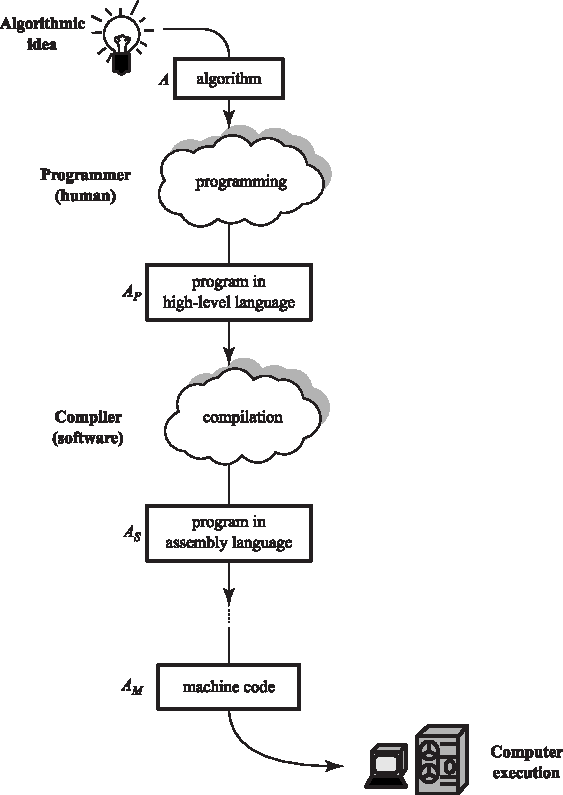
\includegraphics{programming.pdf}
\caption{Proces provedení algoritmu počítačem \citep[s.~56]{spirit}} \label{provedeni2}
\end{figure}

% podkapitola  Programovací paradigmata
% **********************
\section{Programovací paradigmata}
V~jistém smyslu můžeme na informatiku nahlížet jako na vědu, která se zabývá vytváření realizovatelných modelů. Proces vytváření modelů se dá popsat jako relace R(S,P,T,M), kde subjekt S~vytváří model M podle originálu T za účelem P \citep*[s.~135]{didaktikderinformatik}. Jelikož pomocí počítače modelujeme mnoho různých situací, existuje mnoho programovacích jazyků. Ty se sdružují do několika hlavních stylů, které se liší přístupem k~abstrakci dat a operacím s~nimi a představuji specifický přístup k~programu a jeho provedení. Takovéto styly nazýváme programovací paradigmata \citep*[s.~286]{bolshakova}.
\begin{figure}[h!]
\centering
\tikzset{every picture/.append style={font=\fontsize{9}{12}\selectfont}}

\begin{tikzpicture}[node distance=2.5cm]
 \node (start) [startstop] {subjekt \\ S};
  \node (m2) [io,right of=start,yshift=1.5cm] {model \\ M};
  \node (m3) [io,left of=start,yshift=1.5cm] {original \\ T};
\node (v1) [decision,below of=start,yshift=0.7cm] {účel \\ P};
\draw [arrow] (start) -- (m2);
\draw [arrow] (start) -- (m3);
\draw [arrow] (start) -- (v1);
  \end{tikzpicture}
\caption{Schéma vytváření modelů \citep*[s.~135]{didaktikderinformatik}} \label{modely}
\end{figure}

\textbf{Imperativní paradigma} se vyvinulo z~nižších jazyků -- strojového a jazyku symbolických adres \citep*[s.~286]{bolshakova}. Z~pohledu toho paradigmatu je počítač soubor paměťových buněk organizovaných  do různých typů datových struktur, jako pole nebo seznam.  Program v~tomto paradigmatu je sekvence přesných příkazů, která mění data v~těchto strukturách a které jsou spuštěny v~přesném sledu. Jelikož program pracuje se stále stejným paměťovým místem, ke kterému uživatel přistupuje pomocí tzv. proměnných, měl by mít programátor v~každém kroku programu přehled, jak se tyto hodnoty mění. 

Ve \textbf{Funkcionálním paradigmatu}
je programem výraz, který se skládá z~funkcí s~podobnou strukturou jako mají funkce matematické. Jedna funkce může být argumentem jiné funkce. Po spuštění proběhne zjednodušení tohoto výrazu až do podoby, kdy zjednodušit dále nelze.  Neexistuje zde princip modifikovatelné paměti jako v~imperativním paradigmatu \citep*{skavrda}. 

V~\textbf{logickém paradigmatu} je program brán jako soubor logických formulí -- axiomů, které popisují vztahy a vlastnosti nějakých objektů a dotaz, který má být na základě těchto pravidel zodpovězen -- dokázán. 

Základní myšlenka \textbf{objektově orientovaného paradigmatu} se zakládá na představě, že reálný svět je množství objektů, které spolu navzájem komunikují. Definujeme zde skupiny prvků s~podobnými vlastnostmi nazýváme třídy. Na rozdíl od imperativního paradigmatu, ve kterém jsou funkce považovány za aktivního činitele modifikujícího pasivně uložená data, objektově orientované paradigma považuje za aktivní v~paměti uložené objekty a za funkce jsou jen pasivní zprávy, které si objekty mezi sebou posílají.
Přehlednou tabulku paradigmat uvádí Bolshakova \citeyearpar[s.~287]{bolshakova}:
{\renewcommand{\arraystretch}{1.4}% for the vertical padding
\begin{table}
\hyphenpenalty=10000
\footnotesize
\center
    \begin{tabular}{L{2cm} L{2cm} L{3cm} L{3cm} L{3cm}}
   \specialrule{.15em}{.05em}{.05em}  \textbf{Paradigma}              & \textbf{Klíčový koncept}    &\textbf{Program }                            & \textbf{Provedení programu} & \textbf{Výsledek }                    \\ \specialrule{.15em}{.05em}{.05em} 
    Imperativní           & Příkaz (instrukce) & Sekvence příkazů                   & Provedení příkazů           & Zavěrečný stav počítačové paměti \\ \hline
    Funkcionální          & Funkce             & Soubor funkcí                      & Vyhodnocení funkcí          & Hodnota hlavní funkce            \\ \hline
    Logické               & Predikát           & Logické formule: axiomy a theorémy & Logické dokazování theorému & Úspěch nebo neúspěch dokazování \\ \hline
    Objektově orientované & Objekt             & Soubor tříd a objektů              & Výměna zpráv mezi objekty   & Finální stav objektových stavů   \\ \specialrule{.15em}{.05em}{.05em} 
    \end{tabular}
\end{table}

Pro úplnost uveďme ještě tabulku, s~přehledem programovacích jazyků pro příslušná paradigmata. Tato tabulka samozřejmě není úplná, pro každé paradigma najdeme nespočet jazyků, uvádí pouze základní přehled. V~tabulce jsou uvedeny i jazyky, ve kterých můžeme programovat v~několika různých paradigmatech, takové jazyky nazýváme \textbf{multiparadigmatické}. 


\begin{table}[ht]
\hyphenpenalty=10000
\footnotesize
\center
    \begin{tabular}{L{2cm} L{6cm}}
   \specialrule{.15em}{.05em}{.05em}  \textbf{Paradigma}              & \textbf{Klíčový koncept} \\ \specialrule{.15em}{.05em}{.05em} 
    Imperativní           & C, C++, Java, PHP, Python, Ruby\\ \hline
    Funkcionální          & Python, Lisp, Scheme\\ \hline
    Logické               & Prolog  \\ \hline
    Objektově orientované & C++, Java, Python\\ \specialrule{.15em}{.05em}{.05em} 
    \end{tabular}
\end{table}

Je součástí pregraduální přípravy učitelů v~ČR výuka všech paradigmat, nebo se studium zaměřuje pouze na některá? S~kterým paradigmatem se seznámí studenti nejdříve? Jsou pro jednotlivá paradigmata vyhrazeny samostatné předměty, nebo je koncentrovaná výuka více paradigmat do jednoho předmětu? To jsou otázky, které můžeme ve výzkumné části zodpovědět.







%\begin{figure}
%\centering
%   \begin{BVerbatim}
%for (int a = 0; a < 10; a++)
%  for (int b = 0; b < 10; b++) 
 %   ...
%\end{BVerbatim}
%\caption{C++ code}
%\end{figure}
% podkapitola  Programování z pohledu deklarovaného kurikula ZŠ a SŠ
% **********************
\section{Programování z~pohledu deklarovaného kurikula ZŠ a SŠ}
\todo{???tahle kapitola by potřebovala trochu vyladit a zpřehlednit,}\todo{upravit- zavazné není učivo ale výstupy - nutné přepracovat}
Jedním z~určujících dokumentů pro vzdělávání na základních a středních školách je Rámcový vzdělávací program. Tento koncepční dokument určuje a specifikuje obsah výuky na republikové úrovni a odvíjí se od něho dokumenty na úrovni nižší -- školní vzdělávací programy, má tedy zásadní vliv na podobu výuky informatiky v~republice. V~jaké míře je zde programování nebo algoritmizace obsažena? Analyzujme nyní tento dokument, abychom zjistili, zda a jak jsou v~něm témata algoritmizace a programování obsažena. 
 
V~RVP pro základní vzdělávání \citep{rvpzv} spadá pod tzv. vzdělávací oblast Informační a komunikační \textit{Informační a komunikační technologie}. Charakteristika oblasti pojem algoritmus, programování ani jím příbuzná nebo odvozená slova neuvádí. Zaměřuje se spíše na výuku práce s~výpočetní technikou a práci s~informací. Zmínku najdeme tzv. cílových zaměřeních kdy je uvedeno, že \textit{Vzdělání v~oblasti vede žáka k~schopnosti formulovat svůj požadavek a využívat při interakci s~počítačem algoritmické myšlení}. RVP dále kategorizuje vzdělávací obsah a rozděluje ho do učiva prvního a druhého stupně, pojem algoritmizace ani programování zde nenajdeme. 

V~RVP pro gymnázia se mění (rozšiřuje) název vzdělávací oblasti na \textit {Informatika a informační a komunikační technologie}. Jak název napovídá, součástí výuky na gymnáziích by měl být základy informatiky jako vědy. Zaměřuje se hlavně na způsob myšlení \textit {Cílem je zpřístupnit žákům základní pojmy a metody informatiky, napomáhat rozvoji abstraktního, systémového myšlení, podporovat schopnost vhodně vyjadřovat své myšlenky, smysluplnou argumentací je obhajovat a tvůrčím způsobem přistupovat k~řešení problémů.} Pojem algoritmus se tu objevuje už explicitně také \textit {Žák se seznámí se základními principy fungování prostředků ICT a soustředí se na pochopení podstaty a průběhu informačních procesů, algoritmického přístupu k~řešení úloh a významu informačních systémů ve společnosti.} I~mezi cíli je algoritmizace zastoupena a to přímo jako bod \textit {uplatňování algoritmického způsobu myšlení při řešení problémových úloh}. Za cíl, který by se k~algoritmizaci a programování mohl vztahovat také je \textit {porozumění základním pojmům a metodám informatiky jako vědního oboru a k~jeho uplatnění v~ostatních vědních oborech a profesích}, tento bod můžeme reprezentovat mnoha způsoby. Ve vzdělávacím obsahu se pak objevuje tématický okruh \textit {Zpracování  a prezentace informací}, kde jedním z~očekávaných výstupu je, že žák \textit {aplikuje algoritmický přístup k~řešení problémů}. To reflektuje i učivo (které je pro tvorbu ŠVP závazné) a jeho bod \textit {algoritmizace úloh – algoritmus, zápis algoritmu, úvod do programování}, na gymnáziu je tedy výuka programování a algoritmizace \textbf{povinnou součástí}, ale bližší cíle vzdělávání nejsou popsány.\todo{lépe}

Vzdělávání na odborných středních školách probíhá samozřejmě podle RVP také, každý obor má svůj vlastní dokument.  Analyzujme nyní výskyt algoritmizace a programování na RVP oboru Informační technologie \todo{citace}, kde by úroveň informatického vzdělávání měla být nejvyšší z~celého středoškolského systému. Programování najdeme v~tzv. klíčových odborných kompetencích, konkrétně klíčová kompetence Programovat a vyvíjet uživatelská, databázová a webová řešení, tzn. aby absolventi: 
 \begin{itemize}
\setlength\itemsep{0.1em}
\item algoritmizovali úlohy a tvořili aplikace v~některém vývojovém prostředí; 
\item realizovali databázová řešení;  
\item tvořili webové stránky. 
\end{itemize}
 V~RVP pro odborné vzdělávání  existují vzdělávací oblasti tak jako v~RVP pro gymnázia, dělí se ještě dále na tzv. vzdělávací okruhy podle kterých se na školní úrovni definuje obsah jednotlivých předmětů. Pro programování má odborné vzdělávání samostatný okruh nazvaný \textit {programování a vývoj aplikací} jehož cílem je \textit {naučit žáka vytvářet algoritmy a pomocí programovacího jazyka zapsat  zdrojový  kód  programu}. V~tabulce (\ref{table:1}) obsažené v~RVP najdeme definované výsledky vzdělávání a učivo.
%Tabulka odborného vzdělávání
% ***************************
%\setlength{\tabcolsep}{0.9em} % for the horizontal padding
{\renewcommand{\arraystretch}{1.4}% for the vertical padding
\begin{table}[ht]
\hyphenpenalty=10
\footnotesize
\center
\caption{Obsahový okruh \textit {programování a vývoj aplikací}} \label{table:1}
\begin{tabular}{|l|l|}
\hline
% první řádek
Výsledky vzdělávání & Učivo \\\hline
% druhý řádek
  \begin{minipage}[t]{0.45\textwidth}
    Žák:
\begin{itemize}[leftmargin=*,nosep]
  	\item zná vlastnosti algoritmu; 
	\item zanalyzuje úlohu a algoritmizuje ji; 
	\item zapíše algoritmus vhodným způsobem; 
\end{itemize}
  \end{minipage} &
  \begin{minipage}[t]{0.45\textwidth}
\textbf{1 Algoritmizace}
    \begin{itemize}[leftmargin=*,nosep]
  \item význam, prvky algoritmu  
\end{itemize}
  \end{minipage}\\\hline
% 3 řádek
  \begin{minipage}[t]{0.45\textwidth}
\begin{itemize}[leftmargin=*,nosep]
  	\item použije základní datové typy; 
	\item použije řídící struktury programu; 
	\item vytvoří jednoduché strukturované programy;    
\end{itemize}
  \end{minipage} &
  \begin{minipage}[t]{0.45\textwidth}
\textbf{2 Strukturované programování }
    \begin{itemize}[leftmargin=*,nosep]
  \item datové typy
\item řídicí struktury  
\end{itemize}
  \end{minipage}\\\hline
% 4 řádek
  \begin{minipage}[t]{0.45\textwidth}
\begin{itemize}[leftmargin=*,nosep]
  	\item rozumí pojmům třída, objekt a zná jejich základní vlastnosti; 
	\item použije jednoduché objekty; 
\end{itemize}
  \end{minipage} &
  \begin{minipage}[t]{0.45\textwidth}
\textbf{3 Úvod do objektového programování }
    \begin{itemize}[leftmargin=*,nosep]
  \item třída, objekt, vlastnosti tříd
\end{itemize}
  \end{minipage}\\\hline
% 5 řádek
  \begin{minipage}[t]{0.45\textwidth}
\begin{itemize}[leftmargin=*,nosep]
  	\item zná výhody použití jazyka SQL; 
	\item použije základní příkazy jazyka SQL; 
\end{itemize}
  \end{minipage} &
  \begin{minipage}[t]{0.45\textwidth}
\textbf{4 Základy jazyka SQL}
    \begin{itemize}[leftmargin=*,nosep]
  \item základní příkazy (SELECT, UPDATE, INSERT, DELETE)
\end{itemize}
  \end{minipage}\\\hline
% 6 řádek
  \begin{minipage}[t]{0.45\textwidth}
\begin{itemize}[leftmargin=*,nosep]
  	\item aplikuje zásady tvorby WWW stránek; 
	\item orientuje se ve struktuře HTML stránky;
  	\item vytvoří webové stránky včetně optimalizace a validace; 
	\item použije formuláře a skriptovací jazyk.
\end{itemize}
  \end{minipage} &
  \begin{minipage}[t]{0.45\textwidth}
\textbf{5 Tvorba statických a dynamických webových stránek }
  \end{minipage}\\\hline
\end{tabular}


\end{table}

% ***************************
%Tabulka odborného vzdělávání KONEC
% ***************************


Pro odborné školy je tedy vzdělávací obsah blíže specifokován. Najdeme zde i zmínky o~jednotlivých programovacích paradigmatech. 


Shrňme si, jak je programování a algoritmizace obsažena v~RVP všech stupňů vzdělávání a jaký to má důsledek na výuku.
Celá koncepce RVP dává škole pouze obecný rámec, který by měla dodržovat. Pro jednotlivá témata zde není uvedena časová dotace, což dává možnost upřednostnit některá témata před ostatními. Dále zde nejsou uvedeny metody, které mají být při výuce použity, takže např. algoritmizace může být procvičována mnoha různými způsoby.  Pro programování nejsou na národní úrovni určeny ani doporučeny konkrétní programovací jazyky, kromě odborného vzdělávání není ani určeno, jaké paradigma by mělo být při výuce použito. Mezi základními školami vznikají někdy velké rozdíly, kdy některé ŠVP zahrnují programování (skrze dětské programovací jazyky) na prvním stupni, některé vůbec programování nenasazují.\footnote{Měl jsem osobní zkušenost na dvou základních školách, jedna s~využitím disponibilních hodin vyučovala informatiku během 3.-7. ročníku, kdy už ve třetím ročníku výuka obsahovala dětský programovací jazyk Baltík. Druhá škola měla nejnižší možnou dotaci jednu hodinu pro každý stupeň a o~výuce programování se zde vůbec neuvažovalo, jednalo spíše o~výuku informačních technologií.} Obecně lze říci, že výuka ICT je směřována spíše k~ovládání informačních a komunikačních technologií, než k~práci s~algoritmizací a programováním.

Pokud bychom měli tvořit pregraduální přípravu jen a pouze podle  očekávaných výstupů v~RVP, v~programu pro ZŠ by se výuka programování  nemusela objevit vůbec, stačilo by výuka algoritmizace. V~programu pro SŠ už se zcela jistě programování objevit musí, nejsme ale omezeni konkrétním programovacím jazykem, pouze by měla obsahovat průpravu jak do strukturovaného tak objektově orientovaného paradigmatu, . Pregraduální příprava z~pohledu RVP by také měla obsahovat jak průpravu do paradigmatu strukturovaného programování,tak aby byl absolvent schopen zajistit výuku na střední odborné škole oboru informatika. Takováto pregraduální příprava by ale samozřejmě nedávala studentům VŠ dostatečný vhled do problematiky a nepřipravila by je na možné budoucí změny v~RVP. Můžeme ale konstatovat, že podoba RVP dává jistý prostor fakultám pří připravě programů pro budoucí učitele informatiky. Struktura těchto programů tak může reflektovat pohled fakulty na to, jak podle ní vypadá "kvalifikovaný učitel informatiky" 
\subsection{Deklarované kurikulum výuky informatiky na Slovensku}
Jelikož je informatika mladý obor a změny v~něm opravdu rychlé, kurikulární dokumenty nemusí obsahovat nejaktuálnější trendy v~oboru. Analyzujme  proto zakotvení programování ve slovenských kurikulárních dokumentech. Štátný vzdělávací program je tomu českému velmi podobný, vznikl ale o~trochu později. Porovnání těchto kurikulárních dokumentů  pro úroveň ISCED 1 a 2 provedl Berki \citeyearpar{berki2011}, nedostatečná specifikace vzdělávacího obsahu a absence práce s~informatikou jako vědou a algoritmickým myšlením byly jeho  hlavní zjištění. \citep[s.~36]{berki2011} Obsah učiva informatiky je pro školy úrovně ISCED 1-3 rozdělen do pěti okruhů:
\begin{itemize}
\setlength\itemsep{0.01em}
  	\item Informácie okolo nás
	\item Komunikácia prostredníctvom IKT
  	\item Postupy, riešenie problémov, algoritmické myslenie
	\item Princípy fungovania IKT
	\item Informačná spoločnosť
\end{itemize}

Algoritmizaci se věnuje okruh Postupy, riešenie problémov, algoritmické myslenie, ve kterém jsou dále definovány obsahové a výkonové standardy\footnote{Obsahovým standardem rozumíme obsah probíraného učiva, výkonovým standardem jsou výstupní kompetence absolventa}. Uvádím tabulku (\ref{table:2 }) pro úroveň ISCED3.
% ***************************
%Tabulka ŠVP  z roku 2011
% ***************************
{\renewcommand{\arraystretch}{1.4}% for the vertical padding
\begin{table}[t]
\hyphenpenalty=10
\footnotesize
\center
\caption{Obsahový okruh \textit {Postupy, riešenie problémov, algoritmické myslenie } z~ŠVP 2011} \label{table:2 }\todo{citace}
\begin{tabular}{|l|l|}
\hline
\multicolumn{1}{|c|}{Výkonový štandard } & \multicolumn{1}{c|}{Obsahový štandard } \\\hline
%Hľadanie a opravovanie chýb
% **************
\begin{minipage}[t]{0.45\textwidth}
\begin{itemize}[leftmargin=*,nosep]
  	\item Analyzovať problém, navrhnúť algoritmus riešenia problému, zapísať algoritmus
v~zrozumiteľnej formálnej podobe, overiť správnosť algoritmu.
	\item Riešiť problémy pomocou algoritmov, vedieť ich zapísať do programovacieho jazyka,
hľadať a opravovať chyby.
\item Rozumieť hotovým programom, určiť vlastnosti vstupov, výstupov a vzťahy medzi
nimi, vedieť ich testovať a modifikovať.

\item Riešiť úlohy pomocou príkazov s~rôznymi obmedzeniami pouţitia príkazov,
premenných, typov a operácií.
\item Používať základné typy používaného programovacieho jazyka
\item Rozpoznať a odstrániť syntaktické chyby, opraviť chyby vzniknuté počas behu
programu, identifikovať miesta programu, na ktorých môže dôjsť k~chybám počas
behu programu.

\end{itemize}
  \end{minipage} &
  \begin{minipage}[t]{0.45\textwidth}
\begin{itemize}[leftmargin=*,nosep]
  	\item Problém. Algoritmus.~Algoritmy z~beţného života. Spôsoby zápisu algoritmov.
	\item Etapy riešenia problému – rozbor problému, algoritmus, program, ladenie.
\item Programovací jazyk -- syntax, spustenie programu, logické chyby, chyby počas behu
programu. Pojmy – príkazy (priradenie, vstup, výstup), riadiace štruktúry (podmienené
príkazy, cykly), premenné, typy , množina operácií.
\end{itemize}
 \end{minipage}

\\\hline
\end{tabular}
\end{table}
% ***************************
%Tabulka ŠVP  z roku 2011  KONEC
% ***************************
 Slovenské deklarované kurikulum má tedy pro algoritmizaci vlastní okruh, ve kterém jsou je učivo i výstupní standardy rozepsány mnohem detailněji než v~kurikulu českém. U~programovacího jazyka jasně uvádí, které pojmy by měl žák znát. Stejně ale jako české RVP dává prostor k~případné variaci, nedefinuje paradigma programovacího jazyka ani blíže nespecifikuje programovací jazyky. Jelikož je dodržena jednotná struktura napříč všemi stupni vzdělávání, můžeme snadno identifikovat posuny  v~úrovni vzdělávání pro jednotlivá témata. \citep[s.~85]{berki2016}

Slovensko ale v~inovaci pokračovalo a v~roce 2015 nasadilo Inovovaný štatný vzdělávací program, který všechny oblasti ještě dále specifikuje.   Uveďme nyní jako příklad opět  tabulku s~obsahovými a výkonovými standarty předmětu informatika pro úroveň ISCED3 okruhu  Postupy, riešenie problémov, algoritmické myslenie pro 5.--8. ročník víceletého gymnázia\footnote{Na rozdíl od dokumentu z~roku 2011 je obsah vzdělávání rozdělen na dva celky, 1.-4. a 5.-8. ročník}:\todo{tabulka pro tabulku, bud využít nebo smazat či zkrátit}







% ***************************
%Tabulka štatných vzdělávacích programů 
% ***************************
%ČÁST 1
% ***************************
{\renewcommand{\arraystretch}{1.4}% for the vertical padding
\begin{table}[t]
\hyphenpenalty=10
\footnotesize
\center
\caption{Obsahový okruh \textit {programování a vývoj aplikací}} \label{table:3}
\begin{tabular}{|l|l|}
\hline
% první řádek
\multicolumn{1}{|c|}{Výkonový štandard } & \multicolumn{1}{c|}{Obsahový štandard } \\\hline
\multicolumn{2}{|c|}{Analýza problému}\\\hline
% Analýza problému
% **************
  \begin{minipage}[t]{0.45\textwidth}
Žiak vie/dokáže
\begin{itemize}[leftmargin=*,nosep]
  	\item identifikovať vstupné informácie zo zadania úlohy,
	\item popísať očakávané výstupy, výsledky, akcie,
	\item identifikovať problém, ktorý sa bude riešiť algoritmicky,
	\item formulovať a neformálne (prirodzeným jazykom) vyjadriť ideu
	riešenia,
	\item uvažovať o~vlastnostiach vykonávateľa (napr. korytnačka, grafické
pero, robot, a pod.),
	\item naplánovať riešenie úlohy ako postupnosť príkazov vetvenia
a opakovania
\end{itemize}
  \end{minipage} &
  \begin{minipage}[t]{0.45\textwidth}
Vlastnosti a vzťahy: zadaný problém – vstup – výstup\\
Procesy: rozdelenie problému na menšie časti, syntéza riešenia z~riešení
menších častí, identifikovanie opakujúcich sa vzorov, identifikovanie
miest pre rozhodovanie sa (vetvenie a opakovanie), identifikovanie
všeobecných vzťahov medzi informáciami
    \begin{itemize}[leftmargin=*,nosep]
  \item význam, prvky algoritmu  
\end{itemize}
  \end{minipage}\\\hline
%Jazyk na zápis riešenia
% **************
\multicolumn{2}{|c|}{Jazyk na zápis riešenia}\\\hline
  \begin{minipage}[t]{0.45\textwidth}
\begin{itemize}[leftmargin=*,nosep]
  	\item používať jazyk na zápis algoritmického riešenia problému (použiť
konštrukcie jazyka, aplikovať pravidlá jazyka), 
	\item rozpoznať a odstrániť chyby v~zápise,
	\item vytvárať zápisy a interpretovať zápisy podľa nových stanovených
pravidiel (syntaxe) pre zápis algoritmov.
\end{itemize}
  \end{minipage} &
  \begin{minipage}[t]{0.45\textwidth}
Pojem: program, programovací jazyk
Vlastnosti a vzťahy: zápis algoritmu a vykonanie programu, vstup –
vykonanie programu – výstup/akcia
Procesy: zostavenie programu, identifikovanie, hľadanie, opravovanie
chýb
  \end{minipage}\\\hline
%Pomocou postupnosti príkazov
% **************
\multicolumn{2}{|c|}{Pomocou postupnosti príkazov}\\\hline
\begin{minipage}[t]{0.45\textwidth}
\begin{itemize}[leftmargin=*,nosep]
  	\item riešiť problém skladaním príkazov do postupnosti,
	\item aplikovať pravidlá, konštrukcie jazyka pre zostavenie postupnosti príkazov.
\end{itemize}
  \end{minipage} &
  \begin{minipage}[t]{0.45\textwidth}
Pojmy: príkaz, parameter príkazu, postupnosť príkazov
Vlastnosti a vzťahy: ako súvisia príkazy a výsledok realizácie programu
Procesy: zostavenie a úprava príkazov, vyhodnotenie postupnosti prí-
kazov, úprava sekvencie príkazov (pridanie, odstránenie príkazu, zmena
poradia príkazov)
  \end{minipage}\\\hline
%Pomocou nástrojov na interakciu
% **************
\multicolumn{2}{|c|}{Pomocou nástrojov na interakciu}\\\hline
\begin{minipage}[t]{0.45\textwidth}
\begin{itemize}[leftmargin=*,nosep]
  	\item rozpoznávať situácie, kedy treba získať vstup,
	\item identifikovať vlastnosti vstupnej informácie (obmedzenia, rozsah,
formát),
\item rozpoznávať situácie, kedy treba zobraziť výstup, realizovať akciu,

\item zapisovať algoritmus, ktorý reaguje na vstup,
\item vytvárať hypotézu, ako neznámy algoritmus spracováva zadaný
vstup, ak sú dané páry vstup–výstup/akcia.

\end{itemize}
  \end{minipage} &
  \begin{minipage}[t]{0.45\textwidth}
Vlastnosti a vzťahy: prostriedky jazyka pre získanie vstupu, spracovanie
vstupu a zobrazenie výstupu
Procesy: čakanie na neznámy vstup – vykonanie akcie – výstup, ná-
sledný efekt
  \end{minipage}\\\hline
\end{tabular}
\end{table}


%ČÁST 2
% ***************************
{\renewcommand{\arraystretch}{1.4}% for the vertical padding
{\renewcommand{\arraystretch}{1.4}% for the vertical padding
\begin{table}[t]
\hyphenpenalty=10
\footnotesize
\center
\begin{tabular}{|l|l|}
\hline
%Pomocou premenných
% **************
\multicolumn{2}{|c|}{Pomocou premenných}\\\hline
\begin{minipage}[t]{0.45\textwidth}
\begin{itemize}[leftmargin=*,nosep]
  	\item identifikovať zo zadania úlohy, ktoré údaje musia byť zapamätané,
resp. sa menia (a teda vyžadujú použitie premenných),

	\item riešiť problémy, v~ktorých si treba zapamätať a neskôr použiť
zapamätané hodnoty vo výrazoch,
\item zovšeobecňovať riešenie tak, aby fungovalo nielen s~konštantami
\end{itemize}
  \end{minipage} &
  \begin{minipage}[t]{0.45\textwidth}
Pojmy: premenná, meno (pomenovanie) premennej, hodnota premennej,
operácia (+, -, *, /)
Vlastnosti a vzťahy: pravidlá jazyka pre použitie premennej, meno premennej
– hodnota premennej
Procesy: nastavenie hodnoty (priradenie), zistenie hodnoty (použitie
premennej), zmena hodnoty premennej, vyhodnocovanie výrazu
s~premennými, číslami a operáciami
  \end{minipage}\\\hline
%Pomocou cyklov
% **************
\multicolumn{2}{|c|}{Pomocou cyklov}\\\hline
\begin{minipage}[t]{0.45\textwidth}
\begin{itemize}[leftmargin=*,nosep]
  	\item rozpoznávať opakujúce sa vzory,
	\item rozpoznávať, aká časť algoritmu sa má vykonať pred, počas aj po
skončení cyklu,
\item riešiť problémy, v~ktorých treba výsledok získať akumulovaním
čiastkových výsledkov v~rámci cyklu
\item riešiť problémy, ktoré vyžadujú neznámy počet opakovaní,
\item riešiť problémy, v~ktorých sa kombinujú cykly a vetvenia,
\item stanovovať hranice a podmienky vykonávania cyklov.
\end{itemize}
  \end{minipage} &
  \begin{minipage}[t]{0.45\textwidth}
Pojmy: opakovanie, počet opakovaní, podmienka vykonávania cyklu,
telo cyklu
Vlastnosti a vzťahy: ako súvisí počet opakovaní s~výsledkom, čo platí
po skončení cyklu
Procesy: vyhodnotenie hraníc/podmienky cyklu, vykonávanie cyklu
  \end{minipage}\\\hline
%Pomocou vetvenia
% **************
\multicolumn{2}{|c|}{Pomocou vetvenia}\\\hline
\begin{minipage}[t]{0.45\textwidth}
\begin{itemize}[leftmargin=*,nosep]
  	\item rozpoznávať situácie a podmienky, kedy treba použiť vetvenie,
	\item rozpoznávať, aká časť algoritmu sa má vykonať pred, v~rámci
a po skončení vetvenia
\item riešiť problémy, ktoré vyžadujú vetvenie so zloženými podmienkami
(s~logickými spojkami),
\item riešiť problémy, v~ktorých sa kombinujú cykly a vetvenia.
\end{itemize}
  \end{minipage} &
  \begin{minipage}[t]{0.45\textwidth}
Pojmy: vetvenie, podmienka
Vlastnosti a vzťahy: pravda/nepravda – splnená/nesplnená podmienka
Procesy: zostavovanie a upravovanie vetvenia, vytvorenie podmienky
a vyhodnotenie podmienky s~negáciami a logickými spojkami (a, alebo)
  \end{minipage}\\\hline
%Interpretácia zápisu riešenia
% **************
\multicolumn{2}{|c|}{Interpretácia zápisu riešenia}\\\hline
\begin{minipage}[t]{0.45\textwidth}
\begin{itemize}[leftmargin=*,nosep]
  	\item krokovať riešenie, simulovať činnosť vykonávateľa s~postupnos-
ťou príkazov, s~výrazmi a premennými, s~vetvením a s~cyklami,
	\item vyjadrovať ideu daného návodu (objavovať a vlastnými slovami
popísať ideu zapísaného riešenia – ako program funguje, čo zápis
realizuje pre rôzne vstupy),
\item upraviť riešenie úlohy vzhľadom na rôzne dané obmedzenia,
\item dopĺňať, dokončovať, modifikovať rozpracované riešenie,

\item hľadať vzťah medzi vstupom, algoritmom a výsledkom,
\item uvažovať o~rôznych riešeniach, navrhovať vylepšenie.
\end{itemize}
  \end{minipage} &
  \begin{minipage}[t]{0.45\textwidth}
Vlastnosti a vzťahy: jazyk - vykonanie programu
Procesy: krokovanie, čo sa deje v~počítači v~prípade chyby v~programe
 \end{minipage}
\\\hline
\end{tabular}
\end{table}
\clearpage
%ČÁST 3
% ***************************
{\renewcommand{\arraystretch}{1.4}% for the vertical padding
\begin{table}[t]
\hyphenpenalty=10
\footnotesize
\center
\begin{tabular}{|l|l|}
\hline
%Hľadanie a opravovanie chýb
% **************
\multicolumn{2}{|c|}{Hľadanie a opravovanie chýb}\\\hline
\begin{minipage}[t]{0.45\textwidth}
\begin{itemize}[leftmargin=*,nosep]
  	\item rozpoznávať, že program pracuje nesprávne,
	\item hľadať chybu vo vlastnom, nesprávne pracujúcom programe
a opraviť ju,
\item zisťovať, pre aké vstupy, v~ktorých prípadoch, situáciách program
zle pracuje,

\item uvádzať kontra príklad, kedy niečo neplatí, nefunguje,
\item posúdiť a overiť správnosť riešenia (svojho aj cudzieho),
\item rozlišovať chybu pri realizácii od chyby v~zápise.
\end{itemize}
  \end{minipage} &
  \begin{minipage}[t]{0.45\textwidth}
Vlastnosti a vzťahy: chyba v~postupnosti príkazov (zlý príkaz, chýbajú-
ci príkaz, vymenený príkaz alebo príkaz navyše), chyba vo výrazoch
s~premennými, chyba v~algoritmoch s~cyklami a s~vetvením, chyba pri
realizácii (logická chyba), chyba v~zápise (syntaktická chyba)
Procesy: rozpoznanie chyby, hľadanie chyby
 \end{minipage}

\\\hline
\end{tabular}


\end{table}
% ***************************
%Tabulka štatných vzdělávacích programů  KONEC
% ***************************
Výhodou je, že toto dělení je zachováno pro všechny stupně vzdělávání, snadno se identifikuje posun žáků v~jejich znalostech a dovednostech jak píše Berki \citeyearpar[s.~85]{berki2016}, který uvádí i tabulku posunu pro jednotlivé celky napříč celky. Pro náš celek Algoritmické řešení problému je zajímavé také to, že úzce kopíruje samotný algoritmus vývoje softwaru, můžeme ho tedy zobrazit v~přehledném diagramu (obrázek\ref{picture1}), barevně jsou označené bloky společné pro všechny úrovně vzdělávání: 

% ***************************
%TIKZ návaznost slovenských okruhů
% ***************************
\begin{figure}[h!]
\tikzset{every picture/.append style={font=\fontsize{9}{12}\selectfont}}

\begin{tikzpicture}[node distance=2cm]
 \node (start) [startstop] {analýza problému};
  \node (m2) [io,right of=start,xshift=0.8cm] {jazyk na zápis řešení};
  \node (m3) [io,right of=m2,xshift=0.8cm] {řešení problému pomocí:};
\node (v1) [decision,below of=m3,xshift=3cm,yshift=-1cm] {proměných};
\node (v2) [decision,below of=m3,yshift=-1cm] {větvení};
\node (v3) [decision,below of=m3,xshift=-3cm,yshift=-1cm] {cyklů};
\node (v4) [io,below of=m3,xshift=-6cm,yshift=-1cm] {posloupnosti příkazů};
\node (v5) [decision,below of=m3,xshift=6cm,yshift=-1cm] {interakčních nástrojů};
  \node (m4) [io,right of=m3,xshift=0.8cm] {interpretace a~zápis řešení};
  \node (m5) [io,right of=m4,xshift=0.8cm] {hledání a~opravování chyb};
\draw [arrow] (start) -- (m2);
\draw [arrow] (m2) -- (m3);
\draw [arrow] (m3) -- (m4);
\draw [arrow] (m4) -- (m5);
\draw [arrow2] (m3) -- (v1);
\draw [arrow2] (m3) -- (v2);
\draw [arrow2] (m3) -- (v3);
\draw [arrow2] (m3) -- (v4);
\draw [arrow2] (m3) -- (v5);
  \end{tikzpicture}
\caption{Obsahový okruh \textit {programování a vývoj aplikací}} \label{picture1}
\end{figure}

Slovenské deklarované kurikulum podobně jako to české nespecifikuje konkrétní programovou výbavu nebo programovací paradigma. Na rozdíl od něj ale specifikuje a rozděluje obsah vzdělávání do přehledných a smysluplných kategorií, úroveň dosaženého vzdělání je tím lépe ověřitelná.
 
Pokud budeme předpokládat, že jedním z~determinantů pregraduální přípravy jsou i deklarované kurikulum na národní úrovni, slovenská verze kurikula má se svoji specifikovanější podobou výhodu. Tím, že slovenské kurikulum vymezilo pro algoritmizaci a programování vlastní okruh, dává tomuto tématu vysokou důležitost a bere ho jeho nedílnou součást výuky informatiky na základních a středních školách. 
\todo{zkusit zahrnout i Brity}
% ***************************
%podkapitola Proč učit programování?
% ***************************
\section{Proč učit programování?}

%Ačkoliv mají témata algoritmizace a programování v deklarovaném kurikulu pro ZŠ a SŠ jen velmi malé zastoupení, neznamená to, že jsou českou obornou komunitou zabývající se výukou informatiky opomíjena, naopak  je často předkládána. Analyzujme některé z těchto článku abychom mohli vysledovat směry, kterými se může výuka programování v budocnu ubírat. 
\todo{Chybí citace, je potřeba trošku uhladit}
Programování je běžně součástí  pregraduální  přípravy učitelů \citep{berki2013}, toto téma ale nemá u~studentů velkou oblibou \citep{fojtik2015}. Studenti mají obtíže předměty zaměřené na programování absolvovat,“a proto by se raději ve své budoucí pedagogické praxi výuce programování vyhnuli.“ \citep[s.~54 ]{fojtik2015} Studenti se staví spíše proti výuce programování na základních školách, má být podle nich součásti jen výběrových předmětů na gymnáziích. Uvádí důvody jako:
\vspace{2mm}\begin{itemize}[nosep]
  	\item Výuka programování je příliš složitá pro žáky základních i většiny středních škol,
	\item programovací jazyky jsou nesrozumitelné a žáci by je nezvládli,
	\item vývojové nástroje jsou komplikované a nepřehledné,
	\item výuka programování je časově náročná a nezůstal by čas na důležitější témata,
	\item studenti mají negativní zkušenost s~výukou programování na střední nebo základní škole,
	\item nepotřebujeme tolik programátorů v~praxi.
\end{itemize}
\vspace{2mm}Takovýmto studentům je potřeba objasnit několik důvodů, proč by mohlo a mělo být programování a algoritmizace součástí kurikula jak na vysoké škole tak na nižších stupních.  \citep[s.~54 ]{fojtik2015}
Výuka programování a algoritmizace není příprava na povolaní programátora, ale „Cílem programování ve škole je rozvoj tvořivosti a myšlení . Samotné programování je (skvělým) nástrojem k~dosahování těchto cílů." \citep{lessner2015} Koncepty které se studenti naučí během odborného výkladu mohou na základních a středních školách předávat způsobem, kterému rozumí děti, např. Pomocí dětských programovacích jazyků jako Scratch nebo Logo, případně programovat jednoduché roboty.

Schubert a Schwill \citep{didaktikderinformatik} označili jako základní myšlenky informatiky pojmy algoritmus, jazyk a strukturální rozklad. Programování s~těmito pojmy úzce souvisí, dá se tak označit za jedno z~důležitých témat informatiky a mělo by tak být součástí oboru, který připravuje budoucí učitele informatiky

Ačkoliv v~našem RVP má algoritmizace a programování jen malé zastoupení oproti informačním technologiím zaměřeným uživatelským způsobem, v~zahraničí se situace v~poslední  dobou mění. „V současné době probíhají v~řadě zemí kurikulární reformy, v~nichž se vymezuje a mění postavení informatiky. Kurikulární reforma, v~níž má významné postavení informatická složka, probíhá například v~Polsku, v~Austrálii nebo v~Rusku." \citep{nastartu}. Na Slovensku se setkávají žáci s~informatickými tématy jako algoritmické myšlení procedury a princip fungování digitálních technologii  už od 3. třídy. V~Anglii výuka informatiky probíhá ve specializovaném  předmět Computing,(cas, didaktika inf. Na startu) jehož cílem je rozumět a aplikovat základní principy informatiky, kdy se už žáci na prvním stupni základních škol učí psát jednoduché programy.  \citep{england2013}  Je možné, že se dočkáme v~ČR změny kurikulárních dokumentů tímto směrem, učitelé by na to měli být připraveni.

 Velkým příznivcem programování ve vzdělávání byl Seymour Papert, tvůrce dětského programovacího jazyku LOGO. Ve své knize Mindstorms  \citep{mindstorms}popisuje mnoho výhod, které mají  počítače a programování na vývoj a vzdělávání dětí. Ačkoliv tato kniha vyšla už v~roce 1980, můžeme některé myšlenky označit jako nadčasové\footnote{Pepert úzce spolupracoval i s~Jeanem Piagetem, tvůrcem známe teorie kognitivního vývoje, která se na pedagogických fakultách učí dodnes}. Podle Paperta někteří žáci mají model učení postavené na schématu, ve kterém je výsledek špatně nebo správně, neexistuje jiná možnost. Ale v~programování většinou prvotní verze programu není správně, je potřeba najít a opravit chyby. Při tomto schématu  pak není hlavní otázkou zda je program správně nebo špatně, ale zda je opravitelný. Další výhodou je, že při programování žáci využívají a učí se matematickému jazyku a matematice, ke kterému mají lepší vztah, protože je pro ně matematika využitelný nástroj, ne cíl výuky.

% ***************************
%podkapitola Jak učit programování?
% ***************************


\section{Jak učit programování?}
Zaměřme se nyní, na to jakým způsobem je možné programování vyučovat. "Výuka algoritmizace a programování prochází
v~současné době velkými změnami, které se snaží reagovat na dynamický rozvoj softwarového průmyslu. Dříve využívané metodické postupy, modely vývoje či programovací jazyky nedostačují aktuálním potřebám. \citep{fojtik2013}
 
Většinou probíhá výuka nejprve pomocí procedurálního paradigmatu, během kterého jsou studenti obeznámeni s~datovými typy, vytvářením proměnných, operátorech, cyklech, podmínkách apod. Výuka je úzce spojena se syntaxí jazyka, bez které by se student neobešel.  Až následně se přechází k~výuce objektového programování a pojmům jako třída objekt dědičnost. Jednou z~nevýhod takového přístupu je, že ,,žáci z~tohoto postupu získají pocit, že objektové programování je jen určitá nadstavba jazyka".  \citep{fojtik2013}
Výuka může probíhat i pomocí jiných metodik, představme si krátce některé z~nich:
\begin{description}
\item [Object first] Filozofie této metodiky se snaž studentovi v~první řadě představit důležité koncepty objektově orientovaného programování \todo{citace - stránky blueJ}, aniž by se musel zabývat syntaxí programovacího jazyka. Autoří této metodiky vytvořili vývojové prostředí BlueJ pro objektově  orientovaný programovací jazyk Java. Toto prostředí je jednoduché na ovládání a dokáže vizualizovat třídy programu do diagramu.
\item [Architecture first] Tato metodika se snaží rozšiřovat pojetí Object first, ke které přidává ještě větší důslednost na znalost architektury softwaru, než se přejde k~samotnému kódování programu.
\item [Algorithm first]metodika se snaží zaměřit více pozornosti na vytváření algoritmů, než na jejich následném kódování. Studenti tráví více času navrhováním algoritmu a jejich vizualizaci pomocí vývojových diagramů. Díky tomu by měli být schopni převést problémy reálného světa do podoby algoritmu.
\item [Agilní metodiky] Tento pojem zastřešuje přístup k~vývoji softwaru pomocí několika principů např. "Nejúčinnějším a nejefektnějším způsobem sdělování informací vývojovému týmu z~vnějšku i uvnitř něj je osobní konverzace." nebo "Hlavním měřítkem pokroku je fungující software". Studenti v~tomto přístupu zastávaji roli programátorů, vzájemně diskutují a pracují na návrhu softwaru, ke kterému požívají myšlenkové mapy a následně UML diagramy. Poté se přistupuje k~samotnému programování, při kterém se snaží napsat alespoň malou ale hlavně funkční část kódu, což by je mělo motivovat do další práce. Případné problémy mohou vyřešit v~kooperaci s~ostatními.
\begin{figure}[ht]
    \centering
    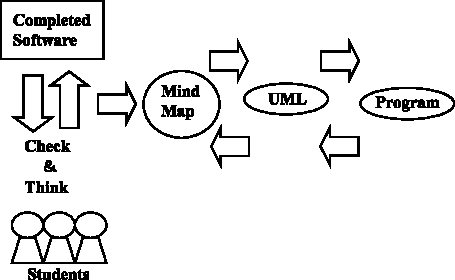
\includegraphics[scale=1.2]{agile.pdf}
\caption{Proces provedení algoritmu počítačem \citep[s.~56]{spirit}} \label{provedeni1}
\end{figure}
\item [Game first] Tato metodika si klade jako prioritu zaujmout studenty. Výuka probíha formou vývoje počítačové hry, při kterém by se měli studenti seznámit i z~odbornými znalostmi programování.
\end{description}
Důležitým aspektem ve výuce programováním je nejen volba  paradigmatu a metodiky, ale i vhodného programovacího jazyka. Milebrandt definoval několik vlastností, které by měl mít programovací jazyk vhodný pro vzdělávání jako například:
\vspace{2mm}\begin{itemize}[nosep]
  	\item jednoduchost použití
	\item jednoduchá syntaxe
	\item dobré testovací nástroje
	\item smysluplné názvy klíčových slov
\end{itemize}
\vspace{2mm}Některé další aspekty definovala Manilla, např.
\vspace{2mm}\begin{itemize}[nosep]
  	\item je zdarma
	\item má širokou podporující komunitu
	\item jeho součástí je dobrý výukový materiál
	\item je rozšiřitelný \ldots
\end{itemize}


\vspace{2mm}Uveďme si nyní několik programovacích jazyků, které jsou v~současnosti relevantní ve výuce programování. Jedná se o~jazyky, které jsou v~českém prostředí známé (články o~nich se objevují ve sbornících odborných konferencí) a jsou vhodné pro výuku programování jak uvádí ve svém výzkumu Manilla  \citeyearpar{mannila}. 
\begin{description}
\item [Python] Jazyk Python byl poprvé vydán v~roce 1991, jeho autorem je Guido Van Rossum. Tento jazyk je interpretovaný a multiparadigmatický, obsahuje konstrukce objektově orientovaného, funkcionálního i imperativního paradigmatu. Jeho výhodou je přehlednost, byl vytvořen s~důrazem na výuku programování. Využívá se k~výuce na předních amerických univerzitách\citeyearpar{guo_2014}. , může být použit i k~výuce na základních školách. "Jazyk sa rýchlo a dobre učí. Programovanie je pragmatické a rýchlo vedie k~stručnému a efektívnemu programovému kódu." \citep{hajek2015}
\item [Java] Java Je objektově orientovaný programovací jazyk, vyvinutý v~roce 1990 Jamesem Gasolinem ve firmě Sun Microsystem. Jeho syntaxe vychází z~populárních jazyků C a C++  \citep{javamanual}. Hojně se využívá i k~výuce programování na vysokých školách. Její výhodou je značná nezávislost na zařízení, je tak využívána např. na mobilních zařízeních jako mobilní telefony nebo tablety. Pro Javu vzniklo několik vývojových prostředí vhodných pro výuku programování, které umožňuj vizualizovat jednotlivé třídy a objekty programu jako např BlueJ  \citep{bluej} nebo Greenfoot \citep{greenfoot}.  
\item [Scratch] Programovací jazyk Scratch je speciálně vytvořen pro výuku dětí. Patří mezi vizuální programovací jazyky, programování tak probíhá manipulací s~grafickými prvky. I~přes svoji jednoduchost dovoluje vytvořit i složitější programátorské konstrukce. Další jeho výhodou je možnost jednoduše sdílet vytvořené projekty v~komunitě. Ačkoliv se nejedná o~klasický, komerčně používaný jazyk, je vhodný k~představení základů a vizualizaci konceptů programování.\citep{scratch}
\item [Scheme] Jazyk Scheme vznikl v~roce 1975, jeho autoři jsou Guy Lewis Steele a Gerald Jay Sussman. Vychází z~programovacího jazyka Lisp, je ale značně zjednodušen,  "je možné syntaxi jazyka Scheme úplně vyložit během jedné přednášky" \citep[s. 11]{scheme}". Jedná se o~multiparadigmatický jazyk, "Jeho podstatou je programovací paradigma funkcionální, je v~něm ale možné pracovat imperativním nebo objektově orientovaným stylem. Scheme je proto často označován jako „algoritmický“ jazyk, tedy jazyk, ve kterém je možno snadno formulovat algoritmy. \citep[s. 10]{scheme}"
\end{description}

V~současnosti může výuka programování probíhat za pomoci mnoha různých programovacích jazyků ,vývojových prostředí a dalších nástrojů např. pro sdílení hotových programů. Každý jazyk, prostředí i nástroj však může mít jiný dopad na rozvoj gramotnosti člověka, jak zmiňují Proctor a Blikstein \citep{proctor2016}. Ti vytvořili tři kategorie, do kterých je jednotlivé jazyky a nástroje možno rozdělit (zestručněno):
\vspace{2mm}\begin{itemize}[nosep]
  	\item materiální -- nástroje, které se soustřeďují hlavně na výuku práce s~kódem
	\item kognitivní -- nástroje, které napomáhají rozvoji rekurzivního a informatického myšlení a abstrakce
	\item sociální -- nástroje, které dovolují využívat kód vytvořený někým dalším nebo se zapojovat do různých komunit
\end{itemize}
Je důležité, aby student učitelství informatiky uvědomoval široké možnosti, jak na své žáky pomocí programování působit a pokud možno udržoval jednotlivé aspekty v~rovnováze, což zmiňuje ve své práci i Kalaš \citep{kalas2016}, který vytvořil rozšířenou verzí didaktického trojúhelníka, ve které rozšiřuje vrchol obsahu na tři podvrcholy -- informatika, oborová didaktika a programovací prostředí. Tyto tři složky by měly být ve výuce stejně zastoupeny, jinak by mohlo podle autora dojít k~deformacím. Pokud se obsah zaměřuje hlavně na programovací prostředí, může to vést k~"technocentrizmu", pokud převládá informatická složka, Kalaš ji doslova označuje jako "Computer Sience centrizmus", což popisuje jako přehnanou snahu zpopularizovat obor informatika na úkor zbylých dvou složek. Nakonec preference didaktického obsahu může vést k~"plytkému nebo žádnému porozumění programovacích konstruktů".\todo{Dopsat že kvůli tomu by určitě měla být součástí didaktika informatiky}
\begin{figure}
    \centering
    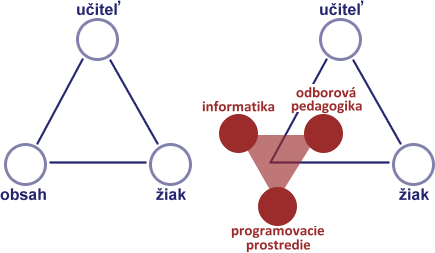
\includegraphics[width=100mm,scale=0.8]{kalas.png}
\caption{Proces provedení algoritmu počítačem \citep[s.~56]{spirit}} \label{provedeni3}
\end{figure}

Pokud bereme v~potaz vše výše uvedené, je zřejmé, že teorie výuky programování dosahuje značné šíře. Aby si byl budoucí učitel informatiky mohl být vědom možností a potencionálních problémů, které výuka programování může představovat, považuji za nutné, aby studenti byly obeznámeni s~didaktikou programování a to nejlépe v~samostatném předmětu.  Jen tak budou moci studenti chápat i další souvislosti výuky programování, protože například jak píše Lessner \citep[s. 13]{lessner2013} "Programování jako takové (vývoj softwaru, popř. zápis algoritmů) ale na gymnáziu těžko obstojí v~roli vzdělávacího cíle. Tímto cílem může být
kultivace myšlení, rozvoj schopnosti systematicky analyzovat a řešit problémy, nikoliv znalost konkrétního programovacího jazyka. Proto by i výuka programování by měla brát v~první řadě důraz na pochopení algoritmů před důkladnou znalostí syntaxe jazyka.
\todo{mozno se ještě dale oprit o~clanek Kalase o~didkatice programování z~Didinfa 2009}
\chapter{Analýza deklarovaného kurikula pregraduální přípravy}
Příprava budoucích učitelů informatiky probíhá v~ČR na přírodovědných a a pedagogických fakultách v~rámci strukturovaných dvoustupňových programů. V~rámci praktického výzkumu byla nejdříve provedena rešerše zdrojů týkajících se této problematiky, následně byla proveden vlastní výzkum skládající se z~vyhledání všech dostupných programů pro pregraduální přípravu učitelů informatiky, vyhledání a kategorizace předmětů zaměřených na programování a algoritmizaci a jejich následná textová analýza. V~každé části výzkumu je popsána příslušná metodika.

\section{Stav problematiky}
V~roce 2013 analyzoval programy pro pregraduální přípravu učitelů informatiky Berki. Byla provedeno porovnání akreditovaných programů  hlavně z~hlediska poměru počtu kreditů pro předem definované kategorie (matematika, algoritmy, databázové a operační systémy, publikační systémy, technologie počítačů, didaktika). Podle této studie bakalářské programy zaměřují spíše na odbornou informatiku, zatímco navazující magisterské programy se zaměřují spíše na didaktiku informatiky. 

\section{Pregradualní příprava učitelů informatiky -- popis zkoumaného vzorku}
Předmětem zkoumání byly studijní programy zaměřené na pregraduální přípravu učitelů informatiky na základních a středních školách. Studie se zaměřuje čistě na prezenční studium, nejsou jde zahrnutý kombinované ani dálkové programy. Pro relevantnost studie byly do výzkumu zahrnuty pouze programy, do kterých jsou přijímáni studenti pro rok 2017/2018. Tímto opatřením bylo tak zajištěno, že budou zahrnuty pouze programy s~platnou akreditací. V~ČR najdeme i některé programy, které spojují informatiku a technickou výchovu, které jsou zaměřeny hlavně pro budoucí učitele odborných středních škol. Tyto programy se značně svým obsahem liší, proto nejsou do studie zahrnuty.
Jelikož mohou vysoké školy akreditovat programy vzdělávající budoucí učitele informatiky akreditovat pod různými jmény, byla provedena rešerše otevíraných oborů na všech fakultách vzdělávajících učitele v~ČR. Z~této rešerše vznikl vzorek 25 studijních programů ze 14 fakult 10 univerzit:\todo{dát oficální názvy nebo nechat názvy s městy?????}
\begin{itemize}
\setlength\itemsep{0.2em}
\item Jihočeská univerzita v Českých Budějovicích (JU) -- Pedagogická fakulta (PedF), Přírodovědecká fakulta (PřF)
\item Masarykova univerzita v Brně (MU) -- Fakulta informatiky (FI)
\item Ostravská univerzita -- Pedagogická fakulta (PedF), Přírodovědecká fakulta (PřF)
\item Technická univerzita v Liberci (TUL) -- Fakulta 	přírodovědně-humanitní a~pedagogická (FPHP)
\item Univerzita Hradec Králové (UHK) -- Přírodovědecká fakulta (PřF), Pedagogická fakulta (PedF)
\item Univerzita Jana Evangelisty Purkyně v Ústí nad Labem (UJEP) -- Přírodovědecká fakulta (PřF)
\item Univerzita Karlova v Praze (UK) -- Matematicko-fyzikální fakulta (MFF), Pedagogická fakulta (PedF)
\item Univerzita Palackého v Olomouci (UP) -- Přírodovědecká fakulta (PřF)
\item Univerzita Tomáše Bati ve Zlíně (UTB) -- Fakulta aplikované informatiky (FAI)
\item Západočeská univerzita v Plzni (ZČU) -- Fakulta pedagogická (PedF)
\end{itemize}
\begin{table}[ht]
\scriptsize
\center
\begin{tabular}{L{1cm} L{4cm} L{1cm}L{5cm}}
\specialrule{.15em}{.05em}{.05em}  \textbf{uni.}              & \textbf{fakulta}    &\textbf{typ }                            & \textbf{program}                   \\ \specialrule{.15em}{.05em}{.05em}
\multirow{4}{*}[-2.2em]{JU}&\multirow{2}{*}[-0.7em]{Pedagogická fakulta}&Bc.& Informační technologie se zaměřením na vzdělávání \\ \cline{3-4}
&&NMgr.&Učitelství informatiky pro 2. stupeň základních škol \\\cline{2-4}
& \multirow{2}{*}[-0.8em]{Přírodovědecká fakulta}&Bc.&Informatika pro vzdělávání \\ \cline{3-4}
&&NMgr.&Učitelství informatiky pro střední školy\\ \hline 
\multirow{2}{*}[-0.8em] {MU} &\multirow{2}{*}[-0.8em] {Fakulta informatiky} &Bc.&Informatika a druhý obor \\ \cline{3-4}
&&NMgr.&Učitelství informatiky pro střední školy\\ \hline
\multirow{3}{*}[-0.8em] {OU} & \multirow{2}{*}[-0.8em] {Přírodovědecká fakulta} &Bc.&Informatika (dvouoborové)\\\cline{3-4}
&&NMgr.&Učitelství informatiky pro 2. stupeň základních škol a střední školy\\\cline{2-4}
& Pedagogická fakulta&Bc.&Informační a komunikační technologie se zaměřením na vzdělávání\\ \hline
\multirow{3}{2cm}[-1.2em]{TUL} &\multirow{3}{4cm}[-1.2em]{Přírodovědně-humanitní
 a~pedagogická}&Bc.&Informatika se zaměřením na vzdělávání\\\cline{3-4}
&&\multirow{2}{2cm}[-0.2em]{NMgr.}&Učitelství informatiky pro střední školy\\\cline{4-4}
&&&Učitelství informatiky pro 2. stupeň základní školy\\ \hline
\multirow{3}{*}[-1.2em] {UHK} &Přírodovědecká fakulta&Bc.&Informatika se zaměřením na vzdělávání\\\cline{2-4}
&\multirow{2}{*}[-0.8em] {Pedagogická fakulta} &\multirow{2}{2cm}[-0.2em]{NMgr.}&Učitelství pro 2. stupeň ZŠ - informatika\\\cline{4-4}
&&&(Učitelství pro střední školy - informatika)\\ \hline
UJEP&  Přírodovědecká fakulta & Bc.                   & Informatika            \\ \hline
\multirow{4}{*}[-0.2em]{UK} &\multirow{2}{*}[-0.2em]{Matematicko-fyzikální fakulta}&Bc.&Informatika se zaměřením na vzdělávání\\ \cline{3-4}
&&NMgr.&Učitelství informatiky\\\cline{2-4}
&\multirow{2}{*}[-0.2em]{Pedagogická fakulta}&Bc.&Informační technologie\\\cline{3-4}
&&NMgr.&Informační a komunikační technologie\\ \hline
\multirow{2}{*}[-0.8em] {UP} & \multirow{2}{*}[-0.8em] {Přírodovědecká fakulta}&Bc.&Informatika pro vzdělávání\\\cline{3-4}
&&NMgr.&Učitelství informatiky pro střední školy\\ \hline
UTB&Fakulta aplikované informatiky&NMgr.&Učitelství informatiky pro střední školy\\ \hline
\multirow{2}{*}[-0.2em] {ZČU}& \multirow{2}{*}[-0.2em] {Fakulta pedagogická}& Bc.& Informatika se zaměřením na vzdělávání\\ \cline{3-4}
&& NMgr.&Učitelství informatiky pro ZŠ\\ \hline
\specialrule{.15em}{.05em}{.05em} 
    \end{tabular}
\end{table}


Pro potřeby studie bylo potřeba vybrat předměty, které souvisí s~výukou programování. V prvním kroku byli analyzovány názvy předmětů v získaných studijních programech a na základě této analýzy a poznatků z teoretické části práce sestavena  množina klíčových slov a sousloví, které by se mohly objevit v názvech předmětů, které souvisí s tématem programování a algoritmizace nebo příbuzných tématech. Tato množina obsahovala např. tyto klíčová slova:\begin{displayquote}
\textit{programování}, \textit{programovací jazyk}, \textit{paradigma}, jména různých programovacích jazyků jako \textit{Java}, \textit{C++}, dále slova související s teorií alogoritmu jako \textit{algoritmus}, \textit{datové struktury}, \textit{složitost}, \textit{vyčíslitelnost}, klíčová slova, která by se mohla objevit v názvu souvisejících s didaktikou programování a robotikou \textit{didaktika}, \textit{robotika} nebo slova, která by mohla souviset s předměty obsahující programovací jazyky určené pro vývoj webových aplikací \textit{www}, \textit{web}.
\end{displayquote}  
Tyto klíčová slova pak byla použita k sestavení prvotní množiny předmětů, do které byly přidány předměty, u kterých z jejich názvů nebylo jasné jejich zaměření a mohli s algoritmizací nebo programováním souviset, např. předmět s názvem \textit{Vstupně výstupní komunikace}. Do studie byly zařazeny výhradně \textbf{povinné} předměty a skupiny povinně volitelných předmětů, kde jsou všechny předměty stejného zaměření, např. když si student musí zvolit z nabídky programovacích předmětů alespoň jeden.
Sylaby předmětů z této prvotní skupiny byly dále podrobnějí zkoumány a  tímto zkoumáním pak předměty rozděleny do čtyř pojmenovaných skupin. Tyto skupiny se dělí podle toho jaká klíčová slova obsahuje části jejich sylabu popísující jednak celkové zaměření předmětu tak i tématický obsah předmětu.

\vspace{2mm}\begin{itemize}
\setlength\itemsep{0.2em}
  	\item \textbf{Výuka programován (VP)í} -- do této kategorie byly zařazeny všechny předměty, jejímž obsahem je výuka konkrétního programovacího jazyka nebo teorie přímo související s~programování jako je teorie paradigmat programování. V sylabech těchto předmětů najdeme klíčové pojmy: \textit{programování}, \textit{programovací jazyk} \textit{programovací paradigma}, názvy konkrétních programovacích paradigmat jako \textit{objektově orientované}, \textit{funkcionální},  názvy konkrétních programovacích jazyků jako \textit{Java}, \textit{C++}.
\item \textbf{Výuka algoritmizace  (VA)} -- do této kategorie jsou zařazeny všechny předměty, jež se zaměřují na výuku teorie algoritmů, datových struktur a teorie složitosti a vyčíslitelnosti algoritmů.. Klíčové pojmy: \textit{algoritmizace}, \textit{algoritmus}, \textit{datové struktury}, \textit{složitost}, \textit{vyčíslitelnost}
\item \textbf{Didaktické předměty (DP)} -- do této kategorie jsou zařazeny předměty, které se zaměřují na didaktiku programování nebo didaktiku algoritmizace, či jsou tato témata obsažena v rámci didaktiky informatiky. Dále jsou zde zaměřeny předměty v nichž je zařazena výuka dětských programovacích jazyků a robotiky\footnote{předpokládá se, že bude robotika představena jako vyučovací nástroj pro výuku didaktiky a algoritmizace}. Klíčové pojmy: \textit{didaktika programování}, \textit{didaktika algoritmizace}, \textit{dětský programovací jazyk}, \textit{robotika}. Jelikož se témata v sylabu mohou mít stejné názvy jako témata ze skupin VP a VA, bude zohledněn i název předmětu.
	\item \textbf{Programování v~prostředí WWW (WWW)} -- do této kategorie jsou zařazeny všechny předměty v nichž se objevuje programování webových aplikací či stránek v některém z programovacích jazyků pro tento účel vhodných. V sylabech těchto předmětů najdeme klíčové pojmy: \textit{PHP}, \textit{JavaScript}, \textit{webová aplikace}, \textit{www}, \textit{web}
\end{itemize}
V případě, že předmět obsahuje klíčové pojmy z více skupin, je zařazen do té, která pokrýva větší část jeho obsahu (je této skupině věnováno více témat). Do statistik je takováto skupina předmětů zařazena ja zahrnuta do statistik v počtu předmětů, které je studen povinen absolovat  Pro zařazení předmětu není dána žádná minimální hranice příslušných pojmů, stačí jediná zmínka vztahující se k jedné ze skupin, aby tento předmět do ni byl zařazen (pokud nejsou přítomna témata z jiných skupin. \textcolor{red}{V průběhu rozřazování bylo zjištěno, že programování a algoritmizace jsou v některých předmětech zastoupeny skoro v rovné míře, což naznačují i poznatky z teoretické části práce. Výuka programování je vlastně "zhmotňování" teorie algoritmů do podoby hotových programů a naopak algoritmy mohou být představeny pomocí programových konstrukcí.}
\begin{figure}[h!]
\centering
\tikzset{every picture/.append style={font=\fontsize{9}{12}\selectfont}}

\begin{tikzpicture}[node distance=2.5cm]
 \node (start) [postup] {krok 1\\získání studijních programů všech oborů};
\node (v1) [postup,below of=start,yshift=0.7cm] {krok 2\\prvotní výběr potencionálně vhodných předmětů na základě výskytu předem definovaných klíčových slov v jejich názvech};
\node (v2) [postup,below of=v1,yshift=0.2cm] {krok 3\\analýza sylabů potencionálně vhodných předmětů a jejich kategorizace na základě výskytu klíčových pojmů v textu zaměření a obsahu těchto předmětů};
\draw [arrow] (start) -- (v1);
\draw [arrow] (v1) -- (v2);
  \end{tikzpicture}
\caption{Metodika výběru předmětů do výzkumu} \label{mode}
\end{figure}

Co je možné porovnat:
\begin{itemize}
\item Porovnání programů hlavně z hlediska programování tedy:
\begin{itemize}
\item porovnání množství předmětů zaměřených na programování
\item porovnání používaných programovacích jazyků
\item porovnání umístění předmětu v rámci studia
\end{itemize}
\item Porovnání didaktiky programování
\begin{itemize}
\item Její výskyt
\item její umístění v rámci studia
\item Její umístění vůči předmětům zaměřených na programování
\end{itemize}


\end{itemize}
\clearpage

\section{Výsledky prvotní analýzy}
Metodikou popsanou výše bylo získáno a kategorizováno celkem 61 předmětů v bakalářských programech studia a 34 předmětů v navazujících  magisterských programech. Data jsou zde prezentována v tabulkách , červeně jsou zvýrazněny položky s nulovým počtem předmětů. 
\subsection{Bakalářské programy}
Získaná data jsou zobrazena v tabulce \ref{my-label}. Podle získaných výsledků jsou bakalářské programy zaměřeny hlavně na výuku programování, na kterou v průměru vymezují 2,08 předmětů v průběhu studia. Výuku programování najdeme až na PedF OU ve všech zkoumaných studijních programech. Jako druhou nejvíce zastoupenou se ukázala výuka algoritmizace zastopena v podobné míře a to s průměrně 2 předměty na studium. Výuka probíhá na všech univerzitách promě PedF UK. Výuka didaktiky programování nebo algoritmizace v bakalářských studijních programech většinou zastoupena, čímž tento výzkum potvrzuje zjištění Berkiho a jeho zjištění, že bakalářské programy se zaměřují převážně na odborné předměty. Vyjímkou je zde výuka na PedF JU, která jako jediná obsahuje dva předměty zaměřené na didaktiku programování nebo algoritmizace. Výuku programovacích jazyků zaměřených na prostředí www většina studijních programů neobsahuje nebo je zastoupena v jednom předmětu. 
Celkově mají bakalářské studijní programy v průměru 4,83 předmětů (medián 4), které spadají do některé z kategorií. Rozdíly mezi programy jsou znatelné --  zatímco na PřF OU vyhovují kriteriům 3 předměty, na PřF UP je to 7 předmětů. Ještě větší rozdíl najdeme, pokud se zaměříme pouze na katogerie VP a VA\footnote{je potřeba zdůraznit, že hranice mezi těmito dvěma kategoriemi je úzká a některé předměty stojí na jejich pomezí -- výuka algoritmizace a programování je zastoupena skoro ve stejné míře}. V tomto případě najdeme  na PedF JU a PedF UK  pouze 2 takto zaměřené předměty, kdežto na PřF UP je těchto předmětů 7, případně 6 na FI MU a MFF UK. Dále je potřeba zmínit že na FI MU a MFF UK je možnost zvolit si vstudovaný programovací jazyk \footnote{to je dáno především velikosti fakult a jejich zaměření i na neučitelské programy studia informatiky}.  Ze získaných dat vyplývá, že dotace hodin  v zkoumané oblasti je pro bakalářské studijní programy rozdílná a to především v předmětech zaměřujících se na výuku algoritmizace a programování.



%{\renewcommand{\arraystretch}{1.2}% for the vertical padding




\todo{Má cenu dělat graf???}
\begin{table}[]
\centering
\scriptsize
\caption{Počet předmětů předmětů v bakalářském studiu}
\label{my-label}
\begin{threeparttable}
\tabcolsep=0.13cm
\begin{tabular}{C{1cm}C{0.7cm}C{0.7cm}C{0.7cm}C{0.7cm}C{0.7cm}C{0.8cm}C{0.7cm}C{0.7cm}C{0.7cm}C{0.7cm}C{0.7cm}C{0.7cm}|>{\columncolor[gray]{.95}[0pt]}C{0.7cm}>{\columncolor[gray]{.95}[0pt]}C{0.7cm}}
\toprule
&PedF JU & PřF JU & FI MU & PřF OU & PedF OU &FP TUL& PřF UHK & PřF UJEP & MFF UK & PedF UK & PřF UP & PedF ZČU& pru& med \\ \midrule
VP&1       & 2      & 3\tnote{1}     & 1      & \textcolor{red}{0}      & 3        &2       & 2        & 3\tnote{2}        &2       & 4      &2&2,08&2        \\ 
VA&1       &2   &3   &2     &3       &1   &2   & 2       &3      &\textcolor{red}{0}       & 3    &2 &2&2      \\ 
DP&2       &\textcolor{red}{0}   &\textcolor{red}{0}   &\textcolor{red}{0}     &\textcolor{red}{0}       &\textcolor{red}{0}   &1   & \textcolor{red}{0}       &\textcolor{red}{0}      &1       &\textcolor{red}{0}    &\textcolor{red}{0} &0,33&0       \\ 
WWW&\textcolor{red}{0}       &1   &\textcolor{red}{0}   &\textcolor{red}{0}     &1       &\textcolor{red}{0}   &1   &\textcolor{red}{0} &\textcolor{red}{0}      &1       & \textcolor{red}{0}    &1&0,42&0        \\ \midrule

celk.&4       &5   &6   &3   &4       &4   &6   & 4       &6      &4       & 7    &5 &4,83&4       \\  \bottomrule
\end{tabular}
\begin{tablenotes}\footnotesize
\item[1] možnost z výběru dvou programovacích jazyků
\item[2] možnost z výběru tří programovacích jazyků
\end{tablenotes}
\end{threeparttable}
\end{table}

\subsection{Navazující magisterské programy}
V navazujících magisterských programech bylo kategorizováno celkem 34 předmětů. Nejvíce jsou zde zastoupeny didaktické předměty s průměrnou dotací 1,46 předmětu na studium. Kromě obou programu PeF UHK je didaktika programování nebo algoritmizace zastoupena v minimálně jednom předmětu. Nejvíce předmětů, jejichž součástí je didaktika programování nebo algoritmizace je obsažena v programu PřF JU.
Druhou nejvíce zastoupenou skupinou jsou předměty na výuku algoritmizace s průměrným zařazením 0,46 předmětu na program, kdy většina fakult ani výuku algoritmizace nezařazuje.
Výuku programování v navazujícím studiu najdeme jen na dvou fakultách -- FAI UTB a FP TUL.  Oba programy FP TUL obsahují dva předměty zaměřené na programování, což je nejvíce ze všech.
V průměru nejméně zastoupenou je výuka programování v prostředí WWW s průměrným výskytem 0,31 předmětu na studijní program. Ve čtyřech studijních programech je do této skupiny zařazen jeden předmět, v ostatních programech toto téma výuky zařazeno není.
Celkově kriteriím některé z kategorií vyhovovalo 2,62 předmětu na studijní program (medián 3).  Při celkovém pohledu na získaná data zjistíme, že v navazujících studijní programy se zaměují hlavně na výuku didaktických témat oproti absenci předmětů z ostatních kategorií. Najdeme zde programy, ve kterých je zastoupena výuka všech kategorií -- FP TUl ZŠ, i program, který nebosahuje žádné předměty zaměřující se na zkoumaná témata.  
\begin{table}[]
\centering
\scriptsize
\caption{Počet předmětů předmětů v NMgr. studiu}
\label{my-label2}
\begin{threeparttable}
\tabcolsep=0.13cm
\begin{tabular}{C{1cm}C{0.7cm}C{0.6cm}C{0.6cm}C{0.6cm}C{0.6cm}C{0.6cm}C{0.7cm}C{0.7cm}C{0.7cm}C{0.7cm}C{0.6cm}C{0.6cm}C{0.7cm}|>{\columncolor[gray]{.95}[0pt]}C{0.7cm}>{\columncolor[gray]{.95}[0pt]}C{0.7cm}}
\toprule
&PedF
JU & PřF JU & FI MU & PřF OU &FP TUL ZŠ&FP TUL SŠ&PedF UHK ZŠ&PedF UHK SŠ&MFF UK&PedF UK&PřF UP&FAI UTB&PedF ZČU&prum&med \\  \midrule
VP	&\cellcolor{red!5}0        &\cellcolor{red!5}0    &\cellcolor{red!5}0    &\cellcolor{red!5}0      &2       &2  &\cellcolor{red!5}0   &\cellcolor{red!5}0        &\cellcolor{red!5}0       &\cellcolor{red!5}0        &\cellcolor{red!5}0     &1  &\cellcolor{red!5}0 &0,38&0    \\ 
VA	&1       &\cellcolor{red!5}0    &\cellcolor{red!5}0    &\cellcolor{red!5}0      &1       &\cellcolor{red!5}0   &\cellcolor{red!5}0    &1       &1      &\cellcolor{red!5}0       &2    &\cellcolor{red!5}0   &\cellcolor{red!5}0   &0,46&0   \\ 
DP	&2       &3   &2   &1     &1       &2   &\cellcolor{red!5}0    & \cellcolor{red!5}0        &2    &1       & 1    &2  &2&1,46&2      \\ 
WWW	&\cellcolor{red!5}0        &\cellcolor{red!5}0    &\cellcolor{red!5}0    &\cellcolor{red!5}0      &1       &1   &\cellcolor{red!5}0   & \cellcolor{red!5}0        &1      &\cellcolor{red!5}0       & \cellcolor{red!5}0     &1  &\cellcolor{red!5}0 &0,31&0     \\ \midrule
celk.&3      &3   &2   &1   &5      &5   &\cellcolor{red!5}0    & 1       &4      &1       &3    &4  &2 &2,62&3     \\  \bottomrule
\end{tabular}
\end{threeparttable}
\end{table}

\subsection{Celkový pohled}

\begin{table}[]
\centering
\scriptsize
\caption{Počet předmětů předmětů v NMgr. studiu}
\label{my-label2}
\begin{threeparttable}
\tabcolsep=0.13cm
\begin{tabular}{C{1cm}C{0.7cm}C{0.6cm}C{0.6cm}C{0.6cm}C{0.6cm}C{0.6cm}C{0.7cm}C{0.7cm}C{0.7cm}C{0.7cm}C{0.6cm}C{0.6cm}C{0.7cm}|>{\columncolor[gray]{.95}[0pt]}C{0.7cm}>{\columncolor[gray]{.95}[0pt]}C{0.7cm}}
\toprule
&PedF
JU & PřF JU & FI MU & PřF OU &FP TUL ZŠ&FP TUL SŠ&PedF UHK ZŠ&PedF UHK SŠ&MFF UK&PedF UK&PřF UP&FAI UTB&PedF ZČU&prum&med \\  \midrule
VP	&\cellcolor{red!5}0        &\cellcolor{red!5}0    &\cellcolor{red!5}0    &\cellcolor{red!5}0      &2       &2  &\cellcolor{red!5}0   &\cellcolor{red!5}0        &\cellcolor{red!5}0       &\cellcolor{red!5}0        &\cellcolor{red!5}0     &1  &\cellcolor{red!5}0 &0,38&0    \\ 
VA	&1       &\cellcolor{red!5}0    &\cellcolor{red!5}0    &\cellcolor{red!5}0      &1       &\cellcolor{red!5}0   &\cellcolor{red!5}0    &1       &1      &\cellcolor{red!5}0       &2    &\cellcolor{red!5}0   &\cellcolor{red!5}0   &0,46&0   \\ 
DP	&2       &3   &2   &1     &1       &2   &\cellcolor{red!5}0    & \cellcolor{red!5}0        &2    &1       & 1    &2  &2&1,46&2      \\ 
WWW	&\cellcolor{red!5}0        &\cellcolor{red!5}0    &\cellcolor{red!5}0    &\cellcolor{red!5}0      &1       &1   &\cellcolor{red!5}0   & \cellcolor{red!5}0        &1      &\cellcolor{red!5}0       & \cellcolor{red!5}0     &1  &\cellcolor{red!5}0 &0,31&0     \\ \midrule
celk.&3      &3   &2   &1   &5      &5   &\cellcolor{red!5}0    & 1       &4      &1       &3    &4  &2 &2,62&3     \\  \bottomrule
\end{tabular}
\end{threeparttable}
\end{table}




\chapter{Textová analýza}
\section{Popis vzorku}
\section{Popis způsobu analýzy}
\section{Výsledky}\todo{Srovnat s~kapitolou 3.1} \todo{Ještě tři podkapitoly:1Jaká je dotace předmětů
Jaká je jejich struktura (jak na sebe navazují, jak jsou oddělené, jestli jsou algoritmy zvlašt nebo dohromady s~programováním)
Obsah předmětů}
\chapter{Návrh konceptu pregraduální přípravy}
\section{ZŠ}
\section{SŠ}
\chapter{Závěr}
\textcolor{gray}{\Blindtext}


\bibliography{citace}

\listoftables

%\begin{quote}
%l,,Programming a computer means nothing more or less than communicating to it in a language
%that it and the human user can both understand. ``\citep{Češka1994}
%\end{quote}
%\chapquote{,,Programming a computer means nothing more or less than \mbox{communicating} to it in a language
%that it and the human user can both understand. ``}{Lewis Carroll}{Alice in Wonderland}
\end{document}
